\documentclass[conference]{IEEEtran}
\IEEEoverridecommandlockouts
% The preceding line is only needed to identify funding in the first footnote. If that is unneeded, please comment it out.
\usepackage{amsmath,amssymb,amsfonts}
\usepackage{algorithmic}
\usepackage{graphicx}
\usepackage[inline, shortlabels]{enumitem}
\usepackage{tabularx}
\usepackage{caption}
\usepackage{titlesec}
\usepackage[T2A,T1]{fontenc}
\usepackage[english]{babel}
\captionsetup{font=it}
\usepackage{ragged2e}
\usepackage{hyperref}
\addto\extrasenglish{%
  \renewcommand{\sectionautorefname}{Section}%
  \renewcommand{\subsectionautorefname}{Subsection}%
  \renewcommand{\subsubsectionautorefname}{Subsubsection}%
  \renewcommand{\tableautorefname}{Table}%
  \renewcommand{\figureautorefname}{Figure}%
}
\usepackage{pifont}
\newcommand{\cmark}{\ding{51}}%
\newcommand{\xmark}{\ding{55}}%
\usepackage{footmisc}
\usepackage{multirow}

% --- Tickz
\usepackage{physics}
\usepackage{amsmath}
\usepackage{tikz}
\usepackage{mathdots}
\usepackage{yhmath}
\usepackage{cancel}
\usepackage{color}
\usepackage{siunitx}
\usepackage{array}
\usepackage{multirow}
\usepackage{amssymb}
\usepackage{gensymb}
\usepackage{tabularx}
\usepackage{extarrows}
\usepackage{booktabs}
\usetikzlibrary{fadings}
\usetikzlibrary{patterns}
\usetikzlibrary{shadows.blur}
\usetikzlibrary{shapes}

% ---------

\usepackage{pdfpages}
\usepackage{booktabs}
\usepackage{csquotes}
\usepackage{lipsum}  
\usepackage{arydshln}
\usepackage{smartdiagram}
\usepackage[inkscapeformat=png]{svg}
\usepackage{textcomp}
\usepackage{tabularray}\UseTblrLibrary{varwidth}
\usepackage{xcolor}
\def\BibTeX{{\rm B\kern-.05em{\sc i\kern-.025em b}\kern-.08em
    T\kern-.1667em\lower.7ex\hbox{E}\kern-.125emX}}
\usepackage{cite}
\usepackage{amsmath}
\newcommand{\probP}{\text{I\kern-0.15em P}}
\usepackage{etoolbox}
\patchcmd{\thebibliography}{\section*{\refname}}{}{}{}

\setlength{\extrarowheight}{2.5pt}

% \renewcommand{\arraystretch}{1.7}

% \setlength{\extrarowheight}{2.5pt}
% \renewcommand{\arraystretch}{0.2}
% \renewcommand{\arraystretch}{1.7}

% --------------
\titleclass{\subsubsubsection}{straight}[\subsection]

\newcounter{subsubsubsection}[subsubsection]
\renewcommand\thesubsubsubsection{\thesubsubsection.\arabic{subsubsubsection}}
\renewcommand\theparagraph{\thesubsubsubsection.\arabic{paragraph}} % optional; useful if paragraphs are to be numbered

\titleformat{\subsubsubsection}
  {\normalfont\normalsize\bfseries}{\thesubsubsubsection}{1em}{}
\titlespacing*{\subsubsubsection}
{0pt}{3.25ex plus 1ex minus .2ex}{1.5ex plus .2ex}

\makeatletter
\renewcommand\paragraph{\@startsection{paragraph}{5}{\z@}%
  {3.25ex \@plus1ex \@minus.2ex}%
  {-1em}%
  {\normalfont\normalsize\bfseries}}
\renewcommand\subparagraph{\@startsection{subparagraph}{6}{\parindent}%
  {3.25ex \@plus1ex \@minus .2ex}%
  {-1em}%
  {\normalfont\normalsize\bfseries}}
\def\toclevel@subsubsubsection{4}
\def\toclevel@paragraph{5}
\def\toclevel@paragraph{6}
\def\l@subsubsubsection{\@dottedtocline{4}{7em}{4em}}
\def\l@paragraph{\@dottedtocline{5}{10em}{5em}}
\def\l@subparagraph{\@dottedtocline{6}{14em}{6em}}
\makeatother

\setcounter{secnumdepth}{4}
\setcounter{tocdepth}{4}
% --------------


\newcommand{\before}[1]{\textcolor{red}{#1}}
\newcommand{\after}[1]{\textcolor{green}{#1}}

\newcommand{\old}[1]{\textcolor{orange}{#1}}
\newcommand{\rem}[1]{\textcolor{red}{#1}}
\newcommand{\todo}[1]{\textcolor{orange}{\newline \textit{\textbf{TODO:} #1}} \newline \newline }

\makeatletter
\newcommand{\linebreakand}{%
  \end{@IEEEauthorhalign}
  \hfill\mbox{}\par
  \mbox{}\hfill\begin{@IEEEauthorhalign}
}
\makeatother




% ---------------------------


\begin{document}

\title{Streamlining Resilient Kubernetes Autoscaling with Multi-Agent Systems via an Automated Online Design Framework\\
    % {\footnotesize \textsuperscript{Note}}
    % \thanks{Identify applicable funding agency here. If none, delete this.}
}

% \IEEEaftertitletext{\vspace{-1\baselineskip}}

\author{

    \IEEEauthorblockN{Julien Soulé}
    \IEEEauthorblockA{\textit{Thales Land and Air Systems, BU IAS}}
    %Rennes, France \\
    \IEEEauthorblockA{\textit{Univ. Grenoble Alpes,} \\
        \textit{Grenoble INP, LCIS, 26000,}\\
        Valence, France \\
        julien.soule@lcis.grenoble-inp.fr}

    \and

    \IEEEauthorblockN{Jean-Paul Jamont\IEEEauthorrefmark{1}, Michel Occello\IEEEauthorrefmark{2}}
    \IEEEauthorblockA{\textit{Univ. Grenoble Alpes,} \\
        \textit{Grenoble INP, LCIS, 26000,}\\
        Valence, France \\
        \{\IEEEauthorrefmark{1}jean-paul.jamont,\IEEEauthorrefmark{2}michel.occello\}@lcis.grenoble-inp.fr
    }

    % \and

    % \IEEEauthorblockN{Michel Occello}
    % \IEEEauthorblockA{\textit{Univ. Grenoble Alpes,} \\
    % \textit{Grenoble INP, LCIS, 26000,}\\
    % Valence, France \\
    % michel.occello@lcis.grenoble-inp.fr}

    % \and

    \linebreakand

    \hspace{-0.5cm}
    \IEEEauthorblockN{Paul Théron}
    \IEEEauthorblockA{
        \hspace{-0.5cm}
        \textit{AICA IWG} \\
        \hspace{-0.5cm}
        La Guillermie, France \\
        \hspace{-0.5cm}
        %lieu-dit Le Bourg, France \\
        paul.theron@orange.fr}

    \and

    \hspace{0.5cm}
    \IEEEauthorblockN{Louis-Marie Traonouez}
    \IEEEauthorblockA{
        \hspace{0.5cm}
        \textit{Thales Land and Air Systems, BU IAS} \\
        \hspace{0.5cm}
        Rennes, France \\
        \hspace{0.5cm}
        louis-marie.traonouez@thalesgroup.com}}


\maketitle

\begin{abstract}
  In cloud-native critical systems relying on complex Kubernetes clusters with interdependent services, poor workload management can jeopardize cluster availability, creating failures possibly exploitable by attackers. Such failures include resource blocking, bottlenecks, and continuous pod crashes. Conventional Horizontal Pod Autoscaling (HPA) approaches often fall short in such dynamic environments, while reinforcement learning-based ones, though more adaptable, typically focus on a single latency or resource minimization objective without explicitly addressing all known failures.
  A Multi-Agent System (MAS) enables resilient Kubernetes HPA by decomposing the availability maximization objective into failure-related sub-objectives delegated to agents. We streamline the generation of such MASs through an online automated framework in four phases: (1) modeling the cluster as a simulation from collected real cluster traces; (2) training agents in simulation, partially guided by roles and missions incorporating knowledge of failures; (3) optionally analyzing the trained agents' behaviors; and (4) transferring the learned behaviors to the real cluster.
  Experimental results show that the generated MASs are original and outperform eight HPA systems as for availability under two clusters with adversarial scenarios.
\end{abstract}

\begin{IEEEkeywords}
    cyberdefense, MARL, Digital Twins, formal
\end{IEEEkeywords}

\section{Introduction}
\label{sec:introduction}

% Contexte
Cloud-native critical systems are increasingly reliant on Kubernetes to orchestrate and manage interdependent services. Horizontal Pod Autoscaling (HPA) is a widely adopted mechanism to dynamically adjust the number of pods based on resource usage, enabling systems to handle highly dynamic workloads. However, failures such as pod crashes, resource contention, and bottlenecks can severely jeopardize cluster availability. Worse, these failures may be exploited by attackers to degrade performance or induce outages, as seen in adversarial contexts like Distributed Denial-of-Service (DDoS) attacks~\cite{KubernetesChallenges, AutoscalingLimitations}.

In such adversarial scenarios, malicious actors often exploit scaling mechanisms, exposing the limitations of conventional HPA systems. Modern approaches have sought to address these gaps using Reinforcement Learning (RL), where an agent optimizes a single global objective such as minimizing latency or resource usage~\cite{SingleObjectiveScaling, RLAutoscalingSurvey}. While these methods demonstrate adaptability, they often fall short in handling diverse failure scenarios. For example, prioritizing responses to cascading pod crashes during an attack may be far more critical than reducing latency under normal conditions. These challenges highlight the need for an autoscaling system capable of dynamically balancing multiple sub-objectives to maximize availability.

Achieving this shift from single-objective optimization to a multi-objective approach is complex, particularly in distributed and dynamic Kubernetes environments. A single-agent RL system struggles to address such complexity due to the difficulty of coordinating responses to diverse and context-dependent failures. In contrast, Multi-Agent Systems (MASs) offer a promising paradigm by decomposing the overarching availability maximization goal into sub-objectives handled by specialized agents~\cite{MultiObjectiveMAS}. Each agent can collaboratively contribute to complementary scaling actions, enabling more resilient and context-specific responses. Our approach builds upon the cyberdefense framework of Autonomous Intelligent Cybersecurity Agents (AICAs)~\cite{kott2018autonomous}, where agents with specialized roles and missions collaboratively defend systems against adversarial threats.

% Problématique
However, designing MASs tailored to Kubernetes clusters presents significant challenges. These include the need for detailed cluster knowledge, the time-consuming nature of manual design processes, and the difficulty of ensuring optimal agent behavior. Additionally, significant cluster changes often necessitate repeating the design process, increasing operational costs and complexity.

% Contribution
Among methdological works, we inspired from the Assisted MAS Organization Engineering Approach (AOMEA)~\cite{soule2024aomea} that shows to align the most with automation and safety challenges. Based on AOMEA, we address these limitations proposing the \textit{Kubernetes Autoscaling with Resilient Multi-Agent systems} (KARMA). This framework automates the design and implementation process through four sequential phases:
\begin{enumerate}
    \item \textbf{Modeling}: Creating a digital twin of the cluster from real-world traces to simulate workload dynamics and failure scenarios.
    \item \textbf{Training}: Training agents in simulation using roles and missions that integrate explicit rule-based strategies.
    \item \textbf{Analyzing}: Validating trained agents' behaviors and extracting design insights through empirical analysis.
    \item \textbf{Transferring}: Deploying trained agents to the real cluster, where they apply their learned behaviors via the Kubernetes API.
\end{enumerate}

This iterative framework continuously updates the simulation model with newly collected traces, enabling adaptation to cluster changes. We validated our approach on two Kubernetes-based environments, "Online Boutique" and "Chained Service," under adversarial scenarios. The MASs were generated with minimal manual intervention, and demonstrate originality and robustness. They consistently outperformed state-of-the-art HPA systems, including AWARE~\cite{AWARE}, Gym-HPA~\cite{GymHPA}, IMAM~\cite{IMAM}, and Libra~\cite{Libra}, in maximizing availability across all evaluated scenarios.

% Organisation
The remainder of this paper is structured as follows:
\autoref{sec:related_work} reviews existing HPA techniques and their limitations in dynamic environments.
\autoref{sec:proposed_approach} details our framework leveraging related concepts for each phase.
\autoref{sec:experiments} describes the experimental setup.
\autoref{sec:results} presents and discusses results.
\autoref{sec:discussion} concludes and provides future directions.

\section{Related Work}
\label{sec:related_work}

\begin{table*}[h!]
  \centering
  \caption{Comparative Study of Autoscaling Systems for Kubernetes HPA}
  \label{tab:autoscaling_criteria}
  \renewcommand{\arraystretch}{1}
  \resizebox{\textwidth}{!}{%
  \begin{tabular}{>{\raggedright\arraybackslash}m{2.5cm}>{\centering\arraybackslash}m{1.5cm}>{\centering\arraybackslash}m{1.5cm}>{\centering\arraybackslash}m{1.5cm}>{\centering\arraybackslash}m{1.5cm}>{\centering\arraybackslash}m{1.5cm}>{\centering\arraybackslash}m{1.5cm}>{\centering\arraybackslash}m{1.5cm}>{\centering\arraybackslash}m{1.5cm}>{\centering\arraybackslash}m{1.5cm}}
  \hline
  \textbf{Criterion} & \textbf{Gym-HPA~\cite{GymHPA}} & \textbf{AWARE~\cite{AWARE}} & \textbf{IMAM~\cite{IMAM}} & \textbf{Libra~\cite{Libra}} & \textbf{QoS-Aware RL~\cite{QoSRL}} & \textbf{AHPA~\cite{AHPA}} & \textbf{KOSMOS~\cite{KOSMOS}} & \textbf{COPA~\cite{COPA}} & \textbf{KARMA} \\
  \hline
  \hline
  Adversarial Scenarios Considered & No & Partial & No & No & No & No & No & Partial & Yes \\
  \hline
  Multi-objective Support & No & Yes & Partial & Indirect & Yes & No & Yes & No & Yes \\
  \hline
  Global Automation Level & High & Middle & Middle & Middle & High & Middle & Middle & Middle & High \\
  \hline
  Learning & Yes & Yes & Yes & Yes & Yes & No & No & No & Yes \\
  \hline
  Multi-Agent System Considered & No & No & Yes & No & No & No & No & No & Yes \\
  \hline
  Simulated Environment & Yes & No & Yes & Yes & Yes & No & No & No & Yes \\
  \hline
  Real Environment & No & Yes & Yes & Yes & Yes & Yes & Yes & Yes & Yes \\
  \hline
  Explainability Considered & No & No & No & No & No & No & No & No & Yes \\
  \hline
  Adaptation Level & High & Middle & High & Middle & Middle & High & High & Middle & High \\
  \hline
  Safety Guarantees & No & No & No & No & No & No & No & No & Yes \\
  \hline
  \end{tabular}%
  }
\end{table*}

Autoscaling in Kubernetes has traditionally relied on metrics-based approaches, such as the default Kubernetes Horizontal Pod Autoscaler (KHPA), which adjusts the number of pods based on CPU and memory utilization~\cite{KubernetesChallenges}. While effective for basic scaling, such methods fail to address dynamic or adversarial workloads, as they rely on reactive, threshold-based rules~\cite{AutoscalingLimitations}. To overcome these limitations, recent research has turned to Machine Learning (ML) and RL.

\subsection*{Reinforcement Learning-Based Systems}
Among RL-based approaches, four systems stand out due to their innovation, applicability, and relevance:

\begin{itemize}
    \item \textbf{Gym-HPA}~\cite{GymHPA} serves as a benchmark RL environment, enabling experimentation with various RL algorithms. It excels in adaptability to simulated workloads with a high degree of automation but lacks multi-objective support, explainability, and real-world applicability.
    \item \textbf{AWARE}~\cite{AWARE} incorporates RL to optimize autoscaling decisions while balancing quality-of-service (QoS) objectives, such as response time and throughput. It partially considers adversarial scenarios but struggles with high automation levels and multi-agent coordination.
    \item \textbf{IMAM}~\cite{IMAM} integrates RL with a multi-agent framework, making it highly adaptive in microservice-based architectures. However, it lacks safety guarantees and explainability, limiting its effectiveness in adversarial contexts.
    \item \textbf{Libra}~\cite{Libra} introduces traffic-aware scaling in edge environments. While it provides valuable insights into traffic optimization, it lacks consideration for multi-objective trade-offs or safety-critical guarantees.
\end{itemize}

These systems highlight significant progress in RL-based autoscaling but share common limitations: a lack of comprehensive adversarial adaptability, limited support for multi-agent systems, and no explicit focus on explainability or safety guarantees.

\subsection*{Hybrid and Rule-Based Approaches}
Other notable systems combine ML or rule-based strategies with traditional autoscaling:

\begin{itemize}
    \item \textbf{QoS-Aware RL}~\cite{QoSRL} focuses on maintaining QoS under dynamic workloads but does not integrate seamlessly with Kubernetes-native features or consider adversarial scenarios.
    \item \textbf{AHPA}~\cite{AHPA} and \textbf{KOSMOS}~\cite{KOSMOS} explore adaptive and combined vertical-horizontal scaling strategies, offering high adaptability but lacking learning capabilities.
    \item \textbf{COPA}~\cite{COPA} emphasizes combined metrics-based autoscaling but remains reactive and limited in adversarial scenarios.
\end{itemize}

\subsection*{Positioning Our Contribution}
Our proposed approach addresses the gaps identified in existing work by introducing an automated MAS framework for Kubernetes HPA, specifically designed to handle adversarial scenarios. \autoref{tab:autoscaling_criteria} provides a comparative overview of key Kubernetes HPA systems with our contribution. Key strengths of our contribution include:
\begin{itemize}
    \item \textbf{Adversarial Scenarios}: Explicit focus on handling attacks like  where conventional autoscaling systems is poorly suited.
    \item \textbf{Multi-Objective Support}: Decomposition of complex objectives (e.g., availability maximization) into agents' missions enabling flexible failure-specific handling.
    \item \textbf{Engineering Automation}: High automation through digital twin modeling and automated MAS generation.
    \item \textbf{Explainability}: Integration of explainability mechanisms to validate agent behavior.
    \item \textbf{Constraint Satisfaction}: Soft and hard constraints can be incorporated in agents through roles, possibly enabling safety guarantees.
    \item \textbf{Adaptability}: Continuous adaptation to workload variations through iterative updates of the digital twin.
\end{itemize}


\section{KARMA: A Framework for MAS-based Kubernetes HPA}
\label{sec:proposed_approach}

This section introduces the KARMA framework as for its global functionning and architectural components.

\subsection{KARMA Overview}

The KARMA framework is designed to address the limitations of conventional HPA by leveraging Multi-Agent Reinforcement Learning (MARL) in a digital twin. Its goal is to provide resilient, explainable, and safe MAS for HPA under adversarial scenarios within an automated development process.

We define resilience through availability maximization which can be defined, in Kubernetes, as the capability of a cluster to efficiently handle user requests at all times while meeting predefined Quality of Service (QoS) contracts~\cite{varghese2019challenges}. We define explainability in a MAS, as the ability of the agents to make decisions at individual or organizational levels that can be understood or expected by humans~\cite{Chakraborti2019Explicability}. We define constraint satisfaction in a MAS as the probability that sequences of actions made by agents do not lead to undesired states which is zero for hard constraints and non-zero for soft ones~\cite{wooldridge2009introduction}. We define engineering automation as  systematic use of methodological tools to autonomously design, implement, validate, and deploy MASs with minimal human intervention~\cite{weyns2020engineering}.

\begin{figure}[h!]
    \centering
    


\tikzset{every picture/.style={line width=0.75pt}} %set default line width to 0.75pt        

\begin{tikzpicture}[x=0.75pt,y=0.75pt,yscale=-1.2,xscale=1.2]
%uncomment if require: \path (0,1414); %set diagram left start at 0, and has height of 1414

%Straight Lines [id:da5609883377896374] 
\draw [color={rgb, 255:red, 74; green, 144; blue, 226 }  ,draw opacity=1 ][line width=2.25]    (317.22,111.13) -- (360.07,111.13) ;
\draw [shift={(365.07,111.13)}, rotate = 180] [fill={rgb, 255:red, 74; green, 144; blue, 226 }  ,fill opacity=1 ][line width=0.08]  [draw opacity=0] (5.72,-2.75) -- (0,0) -- (5.72,2.75) -- cycle    ;
%Image [id:dp9396292457736715] 
\draw (106.77,60.95) node  {
\includegraphics[width=18.66pt,height=18.36pt]{figures/karma_architecture/pod.png}};
%Image [id:dp3874378335758297] 
\draw (145.86,60.95) node  {
\includegraphics[width=18.66pt,height=18.36pt]{figures/karma_architecture/pod.png}};
%Shape: Rectangle [id:dp4562827234223257] 
\draw  [color={rgb, 255:red, 74; green, 144; blue, 226 }  ,draw opacity=1 ][line width=1.5]  (89,28.36) .. controls (89,25.6) and (91.24,23.36) .. (94,23.36) -- (255,23.36) .. controls (257.76,23.36) and (260,25.6) .. (260,28.36) -- (260,132) .. controls (260,134.76) and (257.76,137) .. (255,137) -- (94,137) .. controls (91.24,137) and (89,134.76) .. (89,132) -- cycle ;
%Image [id:dp9455935833751838] 
\draw (172.5,16.24) node  {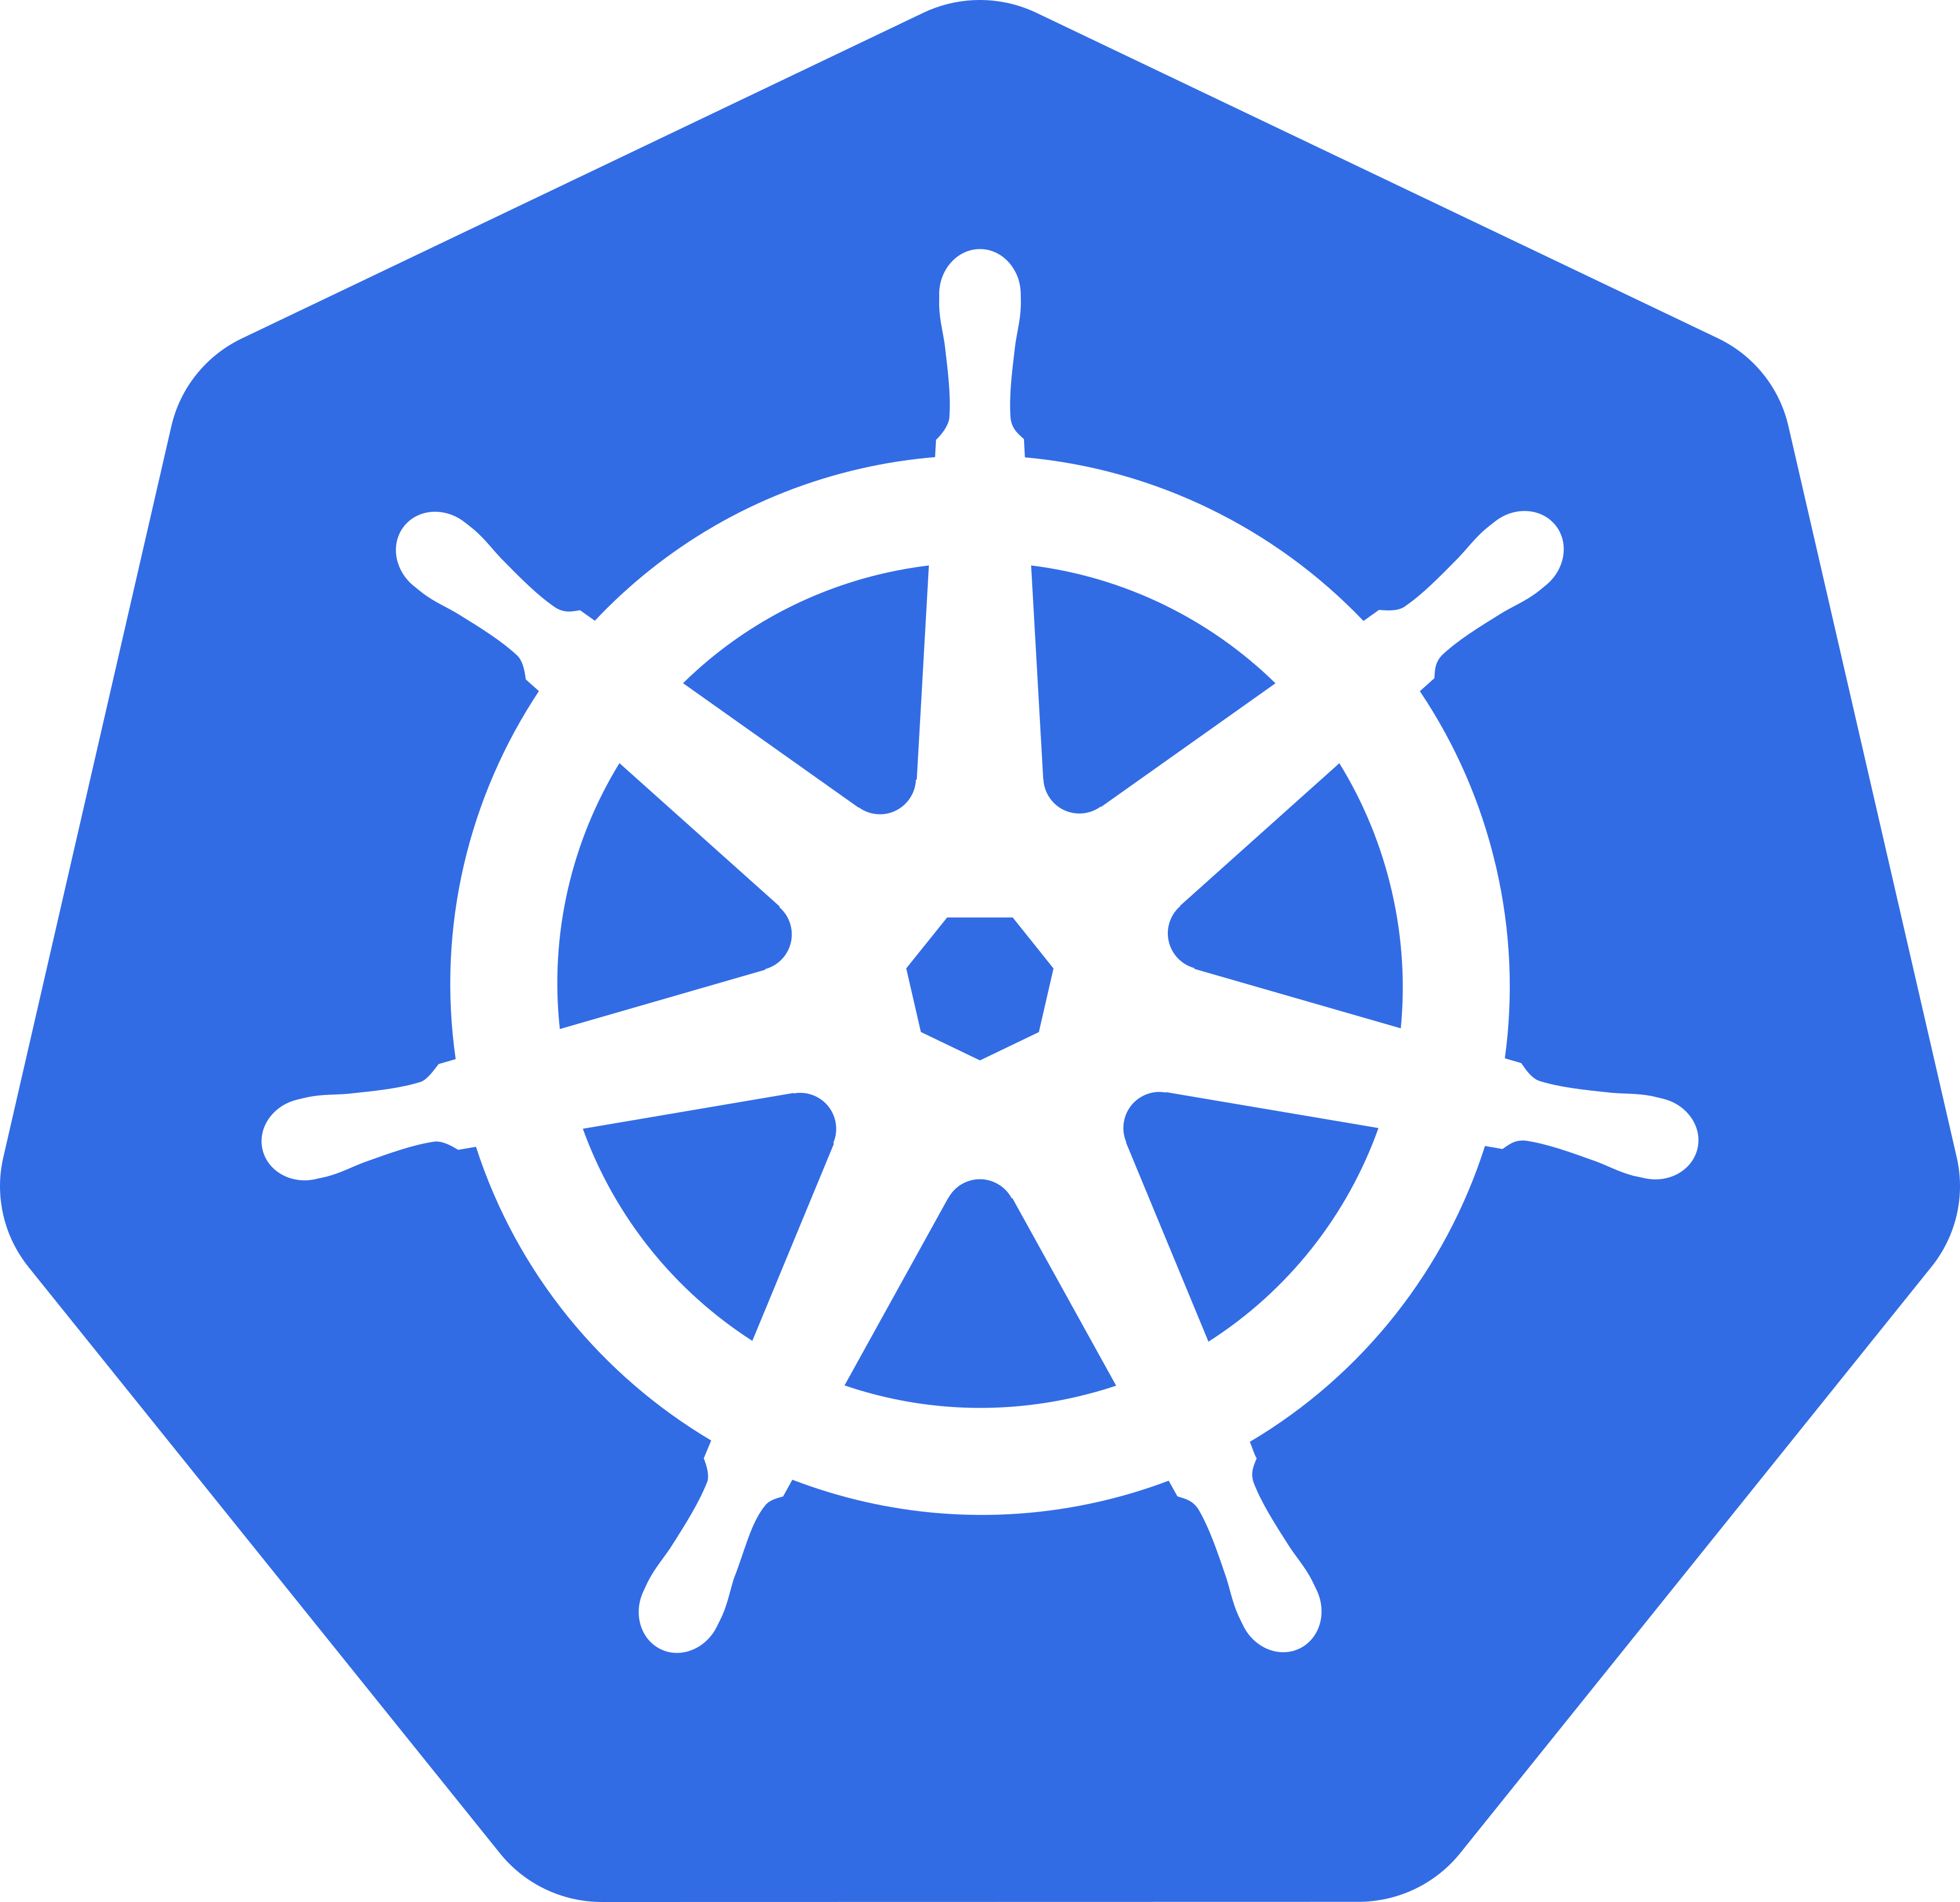
\includegraphics[width=18.66pt,height=18.36pt]{figures/karma_architecture/kubernetes.png}};
%Shape: Rectangle [id:dp9564725691593288] 
\draw  [color={rgb, 255:red, 74; green, 144; blue, 226 }  ,draw opacity=1 ][line width=1.5]  (92.55,50.21) .. controls (92.55,47.45) and (94.79,45.21) .. (97.55,45.21) -- (155.08,45.21) .. controls (157.84,45.21) and (160.08,47.45) .. (160.08,50.21) -- (160.08,70.81) .. controls (160.08,73.57) and (157.84,75.81) .. (155.08,75.81) -- (97.55,75.81) .. controls (94.79,75.81) and (92.55,73.57) .. (92.55,70.81) -- cycle ;
%Image [id:dp9120856447688912] 
\draw (126.32,39.97) node  {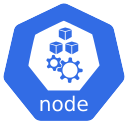
\includegraphics[width=18.66pt,height=18.36pt]{figures/karma_architecture/node.png}};
%Image [id:dp5738167237736518] 
\draw (106.77,119.52) node  {
\includegraphics[width=18.66pt,height=18.36pt]{figures/karma_architecture/pod.png}};
%Image [id:dp2199681121060142] 
\draw (145.86,119.52) node  {
\includegraphics[width=18.66pt,height=18.36pt]{figures/karma_architecture/pod.png}};
%Shape: Rectangle [id:dp12159705904547402] 
\draw  [color={rgb, 255:red, 74; green, 144; blue, 226 }  ,draw opacity=1 ][line width=1.5]  (92.55,108.78) .. controls (92.55,106.02) and (94.79,103.78) .. (97.55,103.78) -- (155.08,103.78) .. controls (157.84,103.78) and (160.08,106.02) .. (160.08,108.78) -- (160.08,129.38) .. controls (160.08,132.14) and (157.84,134.38) .. (155.08,134.38) -- (97.55,134.38) .. controls (94.79,134.38) and (92.55,132.14) .. (92.55,129.38) -- cycle ;
%Image [id:dp37768653229718074] 
\draw (126.32,98.54) node  {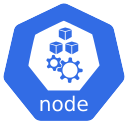
\includegraphics[width=18.66pt,height=18.36pt]{figures/karma_architecture/node.png}};
%Shape: Rectangle [id:dp20840815212238661] 
\draw  [color={rgb, 255:red, 74; green, 144; blue, 226 }  ,draw opacity=1 ][line width=1.5]  (264,28.36) .. controls (264,25.6) and (266.24,23.36) .. (269,23.36) -- (411.78,23.36) .. controls (414.54,23.36) and (416.78,25.6) .. (416.78,28.36) -- (416.78,132) .. controls (416.78,134.76) and (414.54,137) .. (411.78,137) -- (269,137) .. controls (266.24,137) and (264,134.76) .. (264,132) -- cycle ;
%Straight Lines [id:da9232180983272227] 
\draw [color={rgb, 255:red, 74; green, 144; blue, 226 }  ,draw opacity=1 ][line width=2.25]    (164,112) -- (201,112) ;
\draw [shift={(206,112)}, rotate = 180] [fill={rgb, 255:red, 74; green, 144; blue, 226 }  ,fill opacity=1 ][line width=0.08]  [draw opacity=0] (5.72,-2.75) -- (0,0) -- (5.72,2.75) -- cycle    ;
%Straight Lines [id:da6082715106712999] 
\draw [color={rgb, 255:red, 74; green, 144; blue, 226 }  ,draw opacity=1 ][line width=2.25]    (180,90.22) -- (167,90.22) ;
\draw [shift={(162,90.22)}, rotate = 360] [fill={rgb, 255:red, 74; green, 144; blue, 226 }  ,fill opacity=1 ][line width=0.08]  [draw opacity=0] (5.72,-2.75) -- (0,0) -- (5.72,2.75) -- cycle    ;
%Straight Lines [id:da30764510910060716] 
\draw [color={rgb, 255:red, 74; green, 144; blue, 226 }  ,draw opacity=1 ][line width=2.25]    (210,72) -- (199,72) ;
\draw [shift={(194,72)}, rotate = 360] [fill={rgb, 255:red, 74; green, 144; blue, 226 }  ,fill opacity=1 ][line width=0.08]  [draw opacity=0] (5.72,-2.75) -- (0,0) -- (5.72,2.75) -- cycle    ;
%Straight Lines [id:da5394403186779959] 
\draw [color={rgb, 255:red, 74; green, 144; blue, 226 }  ,draw opacity=1 ][line width=2.25]    (178,56.22) -- (167,56.22) ;
\draw [shift={(162,56.22)}, rotate = 360] [fill={rgb, 255:red, 74; green, 144; blue, 226 }  ,fill opacity=1 ][line width=0.08]  [draw opacity=0] (5.72,-2.75) -- (0,0) -- (5.72,2.75) -- cycle    ;
%Straight Lines [id:da6399475815904785] 
\draw [color={rgb, 255:red, 74; green, 144; blue, 226 }  ,draw opacity=1 ][line width=2.25]    (272,72) -- (235,72) ;
\draw [shift={(230,72)}, rotate = 360] [fill={rgb, 255:red, 74; green, 144; blue, 226 }  ,fill opacity=1 ][line width=0.08]  [draw opacity=0] (5.72,-2.75) -- (0,0) -- (5.72,2.75) -- cycle    ;
%Straight Lines [id:da24320102833940327] 
\draw [color={rgb, 255:red, 74; green, 144; blue, 226 }  ,draw opacity=1 ][line width=2.25]    (267,112) -- (230,112) ;
\draw [shift={(272,112)}, rotate = 180] [fill={rgb, 255:red, 74; green, 144; blue, 226 }  ,fill opacity=1 ][line width=0.08]  [draw opacity=0] (5.72,-2.75) -- (0,0) -- (5.72,2.75) -- cycle    ;
%Shape: Rectangle [id:dp9149123987409296] 
\draw  [color={rgb, 255:red, 255; green, 255; blue, 255 }  ,draw opacity=1 ][fill={rgb, 255:red, 255; green, 255; blue, 255 }  ,fill opacity=1 ] (328.83,106.67) -- (353.11,106.67) -- (353.11,114) -- (328.83,114) -- cycle ;
%Image [id:dp7127891043436136] 
\draw (341.68,109.47) node  {
\includegraphics[width=14.57pt,height=15.21pt]{figures/karma_architecture/pettingzoo.png}};
%Straight Lines [id:da5757027637146572] 
\draw [color={rgb, 255:red, 74; green, 144; blue, 226 }  ,draw opacity=1 ][line width=2.25]    (357.9,41) -- (364.9,41) ;
\draw [shift={(352.9,41)}, rotate = 0] [fill={rgb, 255:red, 74; green, 144; blue, 226 }  ,fill opacity=1 ][line width=0.08]  [draw opacity=0] (5.72,-2.75) -- (0,0) -- (5.72,2.75) -- cycle    ;
%Straight Lines [id:da29364722138505184] 
\draw [color={rgb, 255:red, 74; green, 144; blue, 226 }  ,draw opacity=1 ][line width=2.25]    (390.99,97.77) -- (390.99,57.25) ;
\draw [shift={(390.99,52.25)}, rotate = 90] [fill={rgb, 255:red, 74; green, 144; blue, 226 }  ,fill opacity=1 ][line width=0.08]  [draw opacity=0] (5.72,-2.75) -- (0,0) -- (5.72,2.75) -- cycle    ;
%Straight Lines [id:da5470457469462804] 
\draw [color={rgb, 255:red, 74; green, 144; blue, 226 }  ,draw opacity=1 ][line width=2.25]    (390.9,71) -- (325.9,71) ;
\draw [shift={(320.9,71)}, rotate = 360] [fill={rgb, 255:red, 74; green, 144; blue, 226 }  ,fill opacity=1 ][line width=0.08]  [draw opacity=0] (5.72,-2.75) -- (0,0) -- (5.72,2.75) -- cycle    ;
%Shape: Rectangle [id:dp8476965567779329] 
\draw  [color={rgb, 255:red, 255; green, 255; blue, 255 }  ,draw opacity=1 ][fill={rgb, 255:red, 255; green, 255; blue, 255 }  ,fill opacity=1 ] (378.41,65.11) -- (397.83,65.11) -- (397.83,92) -- (378.41,92) -- cycle ;
%Shape: Smiley Face [id:dp8656850497140396] 
\draw  [fill={rgb, 255:red, 255; green, 255; blue, 255 }  ,fill opacity=1 ][line width=0.75]  (380.35,69.4) .. controls (380.35,67.3) and (382.09,65.6) .. (384.24,65.6) .. controls (386.38,65.6) and (388.12,67.3) .. (388.12,69.4) .. controls (388.12,71.5) and (386.38,73.2) .. (384.24,73.2) .. controls (382.09,73.2) and (380.35,71.5) .. (380.35,69.4) -- cycle ; \draw  [fill={rgb, 255:red, 255; green, 255; blue, 255 }  ,fill opacity=1 ][line width=0.75]  (382.53,68.11) .. controls (382.53,67.9) and (382.7,67.73) .. (382.92,67.73) .. controls (383.13,67.73) and (383.31,67.9) .. (383.31,68.11) .. controls (383.31,68.32) and (383.13,68.49) .. (382.92,68.49) .. controls (382.7,68.49) and (382.53,68.32) .. (382.53,68.11) -- cycle ; \draw  [fill={rgb, 255:red, 255; green, 255; blue, 255 }  ,fill opacity=1 ][line width=0.75]  (385.17,68.11) .. controls (385.17,67.9) and (385.34,67.73) .. (385.56,67.73) .. controls (385.77,67.73) and (385.95,67.9) .. (385.95,68.11) .. controls (385.95,68.32) and (385.77,68.49) .. (385.56,68.49) .. controls (385.34,68.49) and (385.17,68.32) .. (385.17,68.11) -- cycle ; \draw  [line width=0.75]  (382.29,70.92) .. controls (383.59,71.94) and (384.88,71.94) .. (386.18,70.92) ;
%Shape: Smiley Face [id:dp9163740789669144] 
\draw  [fill={rgb, 255:red, 255; green, 255; blue, 255 }  ,fill opacity=1 ][line width=0.75]  (392.01,69.4) .. controls (392.01,67.3) and (393.75,65.6) .. (395.89,65.6) .. controls (398.04,65.6) and (399.78,67.3) .. (399.78,69.4) .. controls (399.78,71.5) and (398.04,73.2) .. (395.89,73.2) .. controls (393.75,73.2) and (392.01,71.5) .. (392.01,69.4) -- cycle ; \draw  [fill={rgb, 255:red, 255; green, 255; blue, 255 }  ,fill opacity=1 ][line width=0.75]  (394.18,68.11) .. controls (394.18,67.9) and (394.36,67.73) .. (394.57,67.73) .. controls (394.79,67.73) and (394.96,67.9) .. (394.96,68.11) .. controls (394.96,68.32) and (394.79,68.49) .. (394.57,68.49) .. controls (394.36,68.49) and (394.18,68.32) .. (394.18,68.11) -- cycle ; \draw  [fill={rgb, 255:red, 255; green, 255; blue, 255 }  ,fill opacity=1 ][line width=0.75]  (396.82,68.11) .. controls (396.82,67.9) and (397,67.73) .. (397.21,67.73) .. controls (397.43,67.73) and (397.6,67.9) .. (397.6,68.11) .. controls (397.6,68.32) and (397.43,68.49) .. (397.21,68.49) .. controls (397,68.49) and (396.82,68.32) .. (396.82,68.11) -- cycle ; \draw  [line width=0.75]  (393.95,70.92) .. controls (395.24,71.94) and (396.54,71.94) .. (397.83,70.92) ;
%Shape: Smiley Face [id:dp8186451078369623] 
\draw  [fill={rgb, 255:red, 255; green, 255; blue, 255 }  ,fill opacity=1 ][line width=0.75]  (386.18,77.44) .. controls (386.18,75.34) and (387.92,73.64) .. (390.06,73.64) .. controls (392.21,73.64) and (393.95,75.34) .. (393.95,77.44) .. controls (393.95,79.54) and (392.21,81.24) .. (390.06,81.24) .. controls (387.92,81.24) and (386.18,79.54) .. (386.18,77.44) -- cycle ; \draw  [fill={rgb, 255:red, 255; green, 255; blue, 255 }  ,fill opacity=1 ][line width=0.75]  (388.36,76.15) .. controls (388.36,75.94) and (388.53,75.77) .. (388.74,75.77) .. controls (388.96,75.77) and (389.13,75.94) .. (389.13,76.15) .. controls (389.13,76.36) and (388.96,76.53) .. (388.74,76.53) .. controls (388.53,76.53) and (388.36,76.36) .. (388.36,76.15) -- cycle ; \draw  [fill={rgb, 255:red, 255; green, 255; blue, 255 }  ,fill opacity=1 ][line width=0.75]  (391,76.15) .. controls (391,75.94) and (391.17,75.77) .. (391.39,75.77) .. controls (391.6,75.77) and (391.77,75.94) .. (391.77,76.15) .. controls (391.77,76.36) and (391.6,76.53) .. (391.39,76.53) .. controls (391.17,76.53) and (391,76.36) .. (391,76.15) -- cycle ; \draw  [line width=0.75]  (388.12,78.96) .. controls (389.42,79.98) and (390.71,79.98) .. (392.01,78.96) ;
%Flowchart: Punched Tape [id:dp6020643269389074] 
\draw  [fill={rgb, 255:red, 255; green, 255; blue, 255 }  ,fill opacity=1 ] (313.9,33.81) .. controls (313.9,35.03) and (318.18,36.02) .. (323.45,36.02) .. controls (328.73,36.02) and (333,35.03) .. (333,33.81) .. controls (333,32.58) and (337.28,31.59) .. (342.55,31.59) .. controls (347.83,31.59) and (352.1,32.58) .. (352.1,33.81) -- (352.1,51.52) .. controls (352.1,50.3) and (347.83,49.31) .. (342.55,49.31) .. controls (337.28,49.31) and (333,50.3) .. (333,51.52) .. controls (333,52.75) and (328.73,53.74) .. (323.45,53.74) .. controls (318.18,53.74) and (313.9,52.75) .. (313.9,51.52) -- cycle ;
%Straight Lines [id:da950307097731951] 
\draw [line width=0.75]    (324.14,41.04) -- (341.9,41) ;
%Shape: Smiley Face [id:dp8914579811118104] 
\draw  [line width=0.75]  (320.58,40.88) .. controls (320.58,39.7) and (321.59,38.73) .. (322.85,38.73) .. controls (324.1,38.73) and (325.11,39.7) .. (325.11,40.88) .. controls (325.11,42.07) and (324.1,43.03) .. (322.85,43.03) .. controls (321.59,43.03) and (320.58,42.07) .. (320.58,40.88) -- cycle ; \draw  [line width=0.75]  (321.85,40.15) .. controls (321.85,40.03) and (321.95,39.94) .. (322.08,39.94) .. controls (322.2,39.94) and (322.3,40.03) .. (322.3,40.15) .. controls (322.3,40.27) and (322.2,40.37) .. (322.08,40.37) .. controls (321.95,40.37) and (321.85,40.27) .. (321.85,40.15) -- cycle ; \draw  [line width=0.75]  (323.39,40.15) .. controls (323.39,40.03) and (323.49,39.94) .. (323.62,39.94) .. controls (323.74,39.94) and (323.84,40.03) .. (323.84,40.15) .. controls (323.84,40.27) and (323.74,40.37) .. (323.62,40.37) .. controls (323.49,40.37) and (323.39,40.27) .. (323.39,40.15) -- cycle ; \draw  [line width=0.75]  (321.71,41.74) .. controls (322.47,42.31) and (323.22,42.31) .. (323.98,41.74) ;
%Shape: Smiley Face [id:dp07941198495535606] 
\draw  [line width=0.75]  (329.9,45.15) .. controls (329.9,43.96) and (330.92,43) .. (332.17,43) .. controls (333.42,43) and (334.44,43.96) .. (334.44,45.15) .. controls (334.44,46.33) and (333.42,47.29) .. (332.17,47.29) .. controls (330.92,47.29) and (329.9,46.33) .. (329.9,45.15) -- cycle ; \draw  [line width=0.75]  (331.17,44.42) .. controls (331.17,44.3) and (331.28,44.2) .. (331.4,44.2) .. controls (331.53,44.2) and (331.63,44.3) .. (331.63,44.42) .. controls (331.63,44.54) and (331.53,44.63) .. (331.4,44.63) .. controls (331.28,44.63) and (331.17,44.54) .. (331.17,44.42) -- cycle ; \draw  [line width=0.75]  (332.72,44.42) .. controls (332.72,44.3) and (332.82,44.2) .. (332.94,44.2) .. controls (333.07,44.2) and (333.17,44.3) .. (333.17,44.42) .. controls (333.17,44.54) and (333.07,44.63) .. (332.94,44.63) .. controls (332.82,44.63) and (332.72,44.54) .. (332.72,44.42) -- cycle ; \draw  [line width=0.75]  (331.04,46.01) .. controls (331.79,46.58) and (332.55,46.58) .. (333.3,46.01) ;
%Shape: Smiley Face [id:dp8353415903298282] 
\draw  [line width=0.75]  (341.9,40.85) .. controls (341.9,39.67) and (342.92,38.71) .. (344.17,38.71) .. controls (345.42,38.71) and (346.44,39.67) .. (346.44,40.85) .. controls (346.44,42.04) and (345.42,43) .. (344.17,43) .. controls (342.92,43) and (341.9,42.04) .. (341.9,40.85) -- cycle ; \draw  [line width=0.75]  (343.17,40.12) .. controls (343.17,40) and (343.28,39.91) .. (343.4,39.91) .. controls (343.53,39.91) and (343.63,40) .. (343.63,40.12) .. controls (343.63,40.24) and (343.53,40.34) .. (343.4,40.34) .. controls (343.28,40.34) and (343.17,40.24) .. (343.17,40.12) -- cycle ; \draw  [line width=0.75]  (344.72,40.12) .. controls (344.72,40) and (344.82,39.91) .. (344.94,39.91) .. controls (345.07,39.91) and (345.17,40) .. (345.17,40.12) .. controls (345.17,40.24) and (345.07,40.34) .. (344.94,40.34) .. controls (344.82,40.34) and (344.72,40.24) .. (344.72,40.12) -- cycle ; \draw  [line width=0.75]  (343.04,41.71) .. controls (343.79,42.28) and (344.55,42.28) .. (345.3,41.71) ;
%Straight Lines [id:da21936285199788075] 
\draw [line width=0.75]    (324.19,41.87) -- (329.9,45) ;
%Image [id:dp05694376090002984] 
\draw (218.44,70.24) node  {
\includegraphics[width=18.66pt,height=18.36pt]{figures/karma_architecture/api.png}};
%Image [id:dp7747210194064744] 
\draw (186.74,54.54) node  {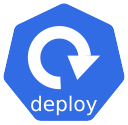
\includegraphics[width=18.66pt,height=18.36pt]{figures/karma_architecture/deploy.png}};
%Image [id:dp5268588430037433] 
\draw (186.74,87.76) node  {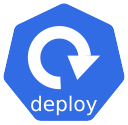
\includegraphics[width=18.66pt,height=18.36pt]{figures/karma_architecture/deploy.png}};
%Image [id:dp7447308292951857] 
\draw (218.44,111.76) node  {
\includegraphics[width=18.66pt,height=18.36pt]{figures/karma_architecture/prometheus.png}};
%Shape: Rectangle [id:dp7837974954754439] 
\draw  [color={rgb, 255:red, 75; green, 101; blue, 225 }  ,draw opacity=1 ][fill={rgb, 255:red, 74; green, 144; blue, 226 }  ,fill opacity=1 ] (202.37,94.64) -- (208.29,94.64) -- (208.29,101.67) -- (202.37,101.67) -- cycle ;
%Shape: Rectangle [id:dp780870970882084] 
\draw  [color={rgb, 255:red, 75; green, 101; blue, 225 }  ,draw opacity=1 ][fill={rgb, 255:red, 74; green, 144; blue, 226 }  ,fill opacity=1 ] (286.37,126) -- (292.29,126) -- (292.29,133.03) -- (286.37,133.03) -- cycle ;

%Shape: Rectangle [id:dp7051683429553395] 
\draw  [color={rgb, 255:red, 75; green, 101; blue, 225 }  ,draw opacity=1 ][fill={rgb, 255:red, 74; green, 144; blue, 226 }  ,fill opacity=1 ] (397.37,124.64) -- (403.29,124.64) -- (403.29,131.67) -- (397.37,131.67) -- cycle ;

%Shape: Rectangle [id:dp5578959475333973] 
\draw  [color={rgb, 255:red, 75; green, 101; blue, 225 }  ,draw opacity=1 ][fill={rgb, 255:red, 74; green, 144; blue, 226 }  ,fill opacity=1 ] (368.37,54.64) -- (374.29,54.64) -- (374.29,61.67) -- (368.37,61.67) -- cycle ;

%Shape: Rectangle [id:dp2822949836407178] 
\draw  [color={rgb, 255:red, 75; green, 101; blue, 225 }  ,draw opacity=1 ][fill={rgb, 255:red, 74; green, 144; blue, 226 }  ,fill opacity=1 ] (324.37,78) -- (330.29,78) -- (330.29,85.03) -- (324.37,85.03) -- cycle ;

%Shape: Rectangle [id:dp9339299822588341] 
\draw  [color={rgb, 255:red, 75; green, 101; blue, 225 }  ,draw opacity=1 ][fill={rgb, 255:red, 74; green, 144; blue, 226 }  ,fill opacity=1 ] (205.37,48) -- (211.29,48) -- (211.29,55.03) -- (205.37,55.03) -- cycle ;



% Text Node
\draw (205.5,98.5) node  [font=\fontsize{0.33em}{0.4em}\selectfont,color={rgb, 255:red, 255; green, 255; blue, 255 }  ,opacity=1 ] [align=left] {1};
% Text Node
\draw (244,58.5) node  [font=\normalsize] [align=left] {{\tiny Scaling}};
\draw (244,64.5) node  [font=\normalsize] [align=left] {{\tiny actions}};
% Text Node
\draw (244,99.5) node  [font=\normalsize] [align=left] {{\tiny Metrics}};
\draw (244,105.5) node  [font=\normalsize] [align=left] {{\tiny data}};
% Text Node
\draw (344.5,36) node  [font=\fontsize{0.33em}{0.4em}\selectfont] [align=left] {\begin{minipage}[lt]{8.66pt}\setlength\topsep{0pt}
\begin{center}
{\fontsize{0.33em}{0.4em}\selectfont $\displaystyle \mathbf{\textcolor[rgb]{0.82,0.01,0.11}{\pi }\textcolor[rgb]{0.82,0.01,0.11}{_{3}}}$}
\end{center}

\end{minipage}};
% Text Node
\draw (341,46.5) node  [font=\fontsize{0.33em}{0.4em}\selectfont] [align=left] {\begin{minipage}[lt]{8.66pt}\setlength\topsep{0pt}
\begin{center}
{\fontsize{0.33em}{0.4em}\selectfont $\displaystyle \mathbf{\textcolor[rgb]{0.82,0.01,0.11}{\pi }\textcolor[rgb]{0.82,0.01,0.11}{_{2}}}$}
\end{center}

\end{minipage}};
% Text Node
\draw (320.9,48) node  [font=\fontsize{0.33em}{0.4em}\selectfont] [align=left] {\begin{minipage}[lt]{8.66pt}\setlength\topsep{0pt}
\begin{center}
{\fontsize{0.33em}{0.4em}\selectfont $\displaystyle \mathbf{\textcolor[rgb]{0.82,0.01,0.11}{\pi }\textcolor[rgb]{0.82,0.01,0.11}{_{1}}}$}
\end{center}

\end{minipage}};
% Text Node
\draw  [color={rgb, 255:red, 75; green, 101; blue, 225 }  ,draw opacity=1 ][fill={rgb, 255:red, 136; green, 197; blue, 246 }  ,fill opacity=1 ][line width=1.5]   (322.77,14.89) .. controls (322.77,13.78) and (323.67,12.89) .. (324.77,12.89) -- (355.77,12.89) .. controls (356.88,12.89) and (357.77,13.78) .. (357.77,14.89) -- (357.77,26.89) .. controls (357.77,27.99) and (356.88,28.89) .. (355.77,28.89) -- (324.77,28.89) .. controls (323.67,28.89) and (322.77,27.99) .. (322.77,26.89) -- cycle  ;
\draw (340.27,20.89) node  [font=\tiny] [align=left] {\begin{minipage}[lt]{21.5pt}\setlength\topsep{0pt}
\begin{center}
KARMA
\end{center}

\end{minipage}};
% Text Node
\draw (290,40.5) node  [font=\tiny] [align=left] {\begin{minipage}[lt]{27.24pt}\setlength\topsep{0pt}
\begin{center}
Organizational\\Analysis
\end{center}

\end{minipage}};
% Text Node
\draw (388,86.39) node  [font=\tiny] [align=left] {\begin{minipage}[lt]{43.42pt}\setlength\topsep{0pt}
\begin{center}
Trained policies
\end{center}

\end{minipage}};
% Text Node
\draw (344.13,127.35) node  [font=\tiny] [align=left] {\begin{minipage}[lt]{60.78pt}\setlength\topsep{0pt}
\begin{center}
PettingZoo environment
\end{center}

\end{minipage}};
% Text Node
\draw (218,127) node  [font=\tiny] [align=left] {\begin{minipage}[lt]{30.31pt}\setlength\topsep{0pt}
\begin{center}
Prometheus
\end{center}

\end{minipage}};
% Text Node
\draw  [color={rgb, 255:red, 75; green, 101; blue, 225 }  ,draw opacity=1 ][fill={rgb, 255:red, 136; green, 197; blue, 246 }  ,fill opacity=1 ][line width=1.5]   (272.9,62) .. controls (272.9,60.9) and (273.8,60) .. (274.9,60) -- (317.9,60) .. controls (319.01,60) and (319.9,60.9) .. (319.9,62) -- (319.9,83) .. controls (319.9,84.1) and (319.01,85) .. (317.9,85) -- (274.9,85) .. controls (273.8,85) and (272.9,84.1) .. (272.9,83) -- cycle  ;
\draw (296.4,72.5) node  [font=\tiny,color={rgb, 255:red, 0; green, 0; blue, 0 }  ,opacity=1 ] [align=left] {Transfer\\Component};
% Text Node
\draw  [color={rgb, 255:red, 75; green, 101; blue, 225 }  ,draw opacity=1 ][fill={rgb, 255:red, 136; green, 197; blue, 246 }  ,fill opacity=1 ][line width=1.5]   (365.88,29.46) .. controls (365.88,28.35) and (366.78,27.46) .. (367.88,27.46) -- (410.88,27.46) .. controls (411.99,27.46) and (412.88,28.35) .. (412.88,29.46) -- (412.88,50.46) .. controls (412.88,51.56) and (411.99,52.46) .. (410.88,52.46) -- (367.88,52.46) .. controls (366.78,52.46) and (365.88,51.56) .. (365.88,50.46) -- cycle  ;
\draw (389.38,39.96) node  [font=\tiny,color={rgb, 255:red, 0; green, 0; blue, 0 }  ,opacity=1 ] [align=left] {Analyzing\\Component};
% Text Node
\draw  [color={rgb, 255:red, 75; green, 101; blue, 225 }  ,draw opacity=1 ][fill={rgb, 255:red, 136; green, 197; blue, 246 }  ,fill opacity=1 ][line width=1.5]   (365.88,98.24) .. controls (365.88,97.13) and (366.78,96.24) .. (367.88,96.24) -- (410.88,96.24) .. controls (411.99,96.24) and (412.88,97.13) .. (412.88,98.24) -- (412.88,119.24) .. controls (412.88,120.34) and (411.99,121.24) .. (410.88,121.24) -- (367.88,121.24) .. controls (366.78,121.24) and (365.88,120.34) .. (365.88,119.24) -- cycle  ;
\draw (389.38,108.74) node  [font=\tiny,color={rgb, 255:red, 0; green, 0; blue, 0 }  ,opacity=1 ] [align=left] {Training\\Component};
% Text Node
\draw (172.5,33.36) node  [font=\tiny] [align=left] {\begin{minipage}[lt]{16.92pt}\setlength\topsep{0pt}
\begin{center}
Cluster
\end{center}

\end{minipage}};
% Text Node
\draw  [color={rgb, 255:red, 75; green, 101; blue, 225 }  ,draw opacity=1 ][fill={rgb, 255:red, 136; green, 197; blue, 246 }  ,fill opacity=1 ][line width=1.5]   (272.9,99) .. controls (272.9,97.9) and (273.8,97) .. (274.9,97) -- (317.9,97) .. controls (319.01,97) and (319.9,97.9) .. (319.9,99) -- (319.9,120) .. controls (319.9,121.1) and (319.01,122) .. (317.9,122) -- (274.9,122) .. controls (273.8,122) and (272.9,121.1) .. (272.9,120) -- cycle  ;
\draw (296.4,109.5) node  [font=\tiny,color={rgb, 255:red, 0; green, 0; blue, 0 }  ,opacity=1 ] [align=left] {Modeling\\Component};
% Text Node
\draw (173,73.72) node  [font=\tiny,rotate=-90] [align=left] {{\LARGE {\fontfamily{helvet}\selectfont \textcolor[rgb]{0.29,0.56,0.89}{...}}}};
% Text Node
\draw (125.61,118.47) node  [font=\tiny] [align=left] {{\LARGE {\fontfamily{helvet}\selectfont \textcolor[rgb]{0.29,0.56,0.89}{...}}}};
% Text Node
\draw (147,89.5) node  [font=\tiny,rotate=-90] [align=left] {{\LARGE {\fontfamily{helvet}\selectfont \textcolor[rgb]{0.29,0.56,0.89}{...}}}};
% Text Node
\draw (125.61,59.9) node  [font=\tiny] [align=left] {{\LARGE {\fontfamily{helvet}\selectfont \textcolor[rgb]{0.29,0.56,0.89}{...}}}};
% Text Node
\draw (208.5,51.86) node  [font=\fontsize{0.33em}{0.4em}\selectfont,color={rgb, 255:red, 255; green, 255; blue, 255 }  ,opacity=1 ] [align=left] {6};
% Text Node
\draw (327.5,81.86) node  [font=\fontsize{0.33em}{0.4em}\selectfont,color={rgb, 255:red, 255; green, 255; blue, 255 }  ,opacity=1 ] [align=left] {5};
% Text Node
\draw (371.5,58.5) node  [font=\fontsize{0.33em}{0.4em}\selectfont,color={rgb, 255:red, 255; green, 255; blue, 255 }  ,opacity=1 ] [align=left] {4};
% Text Node
\draw (400.5,128.5) node  [font=\fontsize{0.33em}{0.4em}\selectfont,color={rgb, 255:red, 255; green, 255; blue, 255 }  ,opacity=1 ] [align=left] {3};
% Text Node
\draw (289.5,129.86) node  [font=\fontsize{0.33em}{0.4em}\selectfont,color={rgb, 255:red, 255; green, 255; blue, 255 }  ,opacity=1 ] [align=left] {2};


\end{tikzpicture}
    \caption{Overview of the KARMA framework in use with a Kubernetes cluster}
    \label{fig:karma_architecture}
\end{figure}

As illustrated in \autoref{fig:karma_architecture}, the KARMA framework operates alongside the Kubernetes cluster, which comprises \textbf{worker nodes} hosting \textbf{pods} that are the atomic unit of work in Kubernetes containing \textbf{containers} that run the actual processes. Pods are labeled into \textbf{services} and managed by \textbf{deployments}.
% TODO: est-ce que ce paragraphe est correct ?
%
The KARMA framework is deployed as an aside software process connected to both the Kubernetes API and Prometheus'one. It consists of four primary components which operate iteratively to optimize the system's scaling policies. The interaction between the Kubernetes cluster and the KARMA framework is overviewed below:

\textbf{1)} \textbf{Metrics Collection:} Metrics related to availability (such as CPU, memory usage, or failed pod number) are continuously collected as states by \textit{Prometheus}~\cite{prometheus}, a widely adopted time-series metrics database, and sent to KARMA's \textbf{Modeling Component}.

\textbf{2)} \textbf{Modeling:} These state are used to construct a \textit{digital twin} of the cluster as a near-realistic state transition function. The reward function is defined as a linear combination of reward sub-function each targeting a known Quality of Service (QoS). Then, we couple the defined reward function for availability to the modeled transition function within a MARL-compatible environment using the PettingZoo library~\cite{Terry2021}.

\textbf{2)} \textbf{Agent Training:} The \textbf{Training Component} uses the modeled environment to train MARL agents, which aim to maximize the cumulative rewards. The reward function encourages scaling policies that improve availability while minimizing resource consumption and latency. Agents are optionally assigned \textit{roles} (rule-based constraints to guide policy exploration) and \textit{missions} (incremental objectives to aid policy convergence), following the methodology proposed by AOMEA~\cite{soule2024aomea}.
    
\textbf{3)} \textbf{Policy Analysis and Explainability:} The \textbf{Analyzing Component} evaluates the behavior of trained agents using trajectory clustering and hierarchical visualization techniques. This ensures that the learned policies are interpretable, aligned with system objectives, and resilient under dynamic workloads or adversarial conditions.
    
\textbf{4)} \textbf{Policy Deployment:} The \textbf{Transfer Component} deploys the trained agents' policies to the real Kubernetes cluster. It sends scaling actions, such as adjusting the number of replicas in a deployment, to the Kubernetes API. These actions are executed in the cluster, completing the iterative feedback loop.

By combining these components, KARMA seamlessly integrates simulation-based learning with real-world Kubernetes operations. Metrics from the cluster inform the policy refinement in the \textbf{Modeling Component}, while scaling decisions derived from trained agents are applied back to the cluster. This closed-loop process ensures continuous improvement, adaptability to workload variations, and robustness against adversarial scenarios.

In the next sub-sections, we will detail each phase of the KARMA framework, including the underlying theoretical concepts and their technical implementation.

\subsection{Phase 1: Modeling}

% Description haut niveau
The modeling phase in the KARMA framework constructs a digital twin of the Kubernetes cluster by leveraging real-world set of state transitions refered to as trajectories, histories, or traces. We envision the environment considering an attacker trying to leverage actions related to data alteration and sheer amount of data to provoke various failures in the cluster, while three to four defender agents would try to manage pod replica in order to minimize the attacker's impact.

This phase uses collected traces to provide a near-realistic simulation environment where the defender agents' policies and the attacker policy can be safely tested and optimized before transfering in the real system. Inspired by the Gym-HPA framework~\cite{GymHPA}, the modeling component employs a state transition model for which we propose to add a deep learning-based approximation of cluster dynamics.

% Formalisation
Even though AOMEA suggests using \textbf{Decentralized Partially Observable Markov Decision Process} (Dec-POMDP) to formalize the environment, it is over-dimmensioned since the environment is fully observable. Therefore, we formalize the environment as a zero-sum \textbf{Stochastic Game (SG)}~\cite{shapley1953stochastic}, which is an extension of the \textbf{Markov Decision Process} (MDP) to multi-agent interactions. The SG is characterized by the tuple $\mathcal{SG} = (\mathcal{A}, S, A, T, R, \gamma)$, where:

\begin{itemize}
  \item $\mathcal{A} = \{\mathcal{A}_d, \mathcal{A}_a\}$ is the agents set comprising $n = |\mathcal{A}_d|$ defender agents and one single attacker agent in $\mathcal{A}_a$;
  \item $S$ is the shared state space characterized by metrics values for both attacker and defender agents;
  \item $A = A_d^n \times A_a$ is the action space with $A_d$ and $A_a$ are the action spaces for a defender and the attacker agents respectively;
  \item $T: S \times A \rightarrow S = S \times A_d^n \times A_a \to S$ is the state transition function dictating the next state when the joint actions of the defender agents and the attacker's one are applied in the environment;
  \item $R = \{R_d, R_a\}$, where $R_d: S \times A_d^n \to \mathbb{R}$ and $R_a: S \times A_a \to \mathbb{R} = - R_d$ are the reward functions for the defender agents and the attacker one respectively;
  \item $\gamma \in [0, 1)$ is the discount factor for future rewards.
\end{itemize}

The following paragraphs detail each component of this formalisation.\\

\noindent \textbf{State Space:} The state of the Kubernetes cluster at time $t$, denoted as $s_t \in S$, consists of metrics critical to characterizing system performance for each of the $d = |D|$ micro-service deployments:
$$
s_t = (n_{id}, d_{dep}, d_{des}, d_{err}, d_{rem}, r_{cpu}, r_{ram}, t_{in}, t_{out})^d
$$
$n_{id} \in \mathbb{N}$: the number of the deployment; \quad
$d_{dep} \in \mathbb{N}$: the number of deployed pods; \quad 
$d_{des} \in \mathbb{N}$: the number of desired pods; \quad
$d_{err} \in \mathbb{N}$: the number of failed pods; \quad
$d_{rem} \in \mathbb{N}$: the number of remaining requests to be processed in the queue; \quad
$r_{cpu} \in \mathbb{R}$: the total aggregated CPU (in m) of the pods; \quad
$r_{ram} \in \mathbb{R}$: the total aggregated memory (in Mi) of the pods; \quad
$t_{in} \in \mathbb{R}$: the average received traffic (in Kbps); \quad
$t_{out} \in \mathbb{R}$: the average transmitted traffic (in Kbps).
% TODO: ajouter les métriques spécifiques pour pouvoir vérifier s'il y a des goulots d'étranglement, 

These metrics are continuously collected using Prometheus~\cite{prometheus}, a widely adopted monitoring and metrics database system, enabling the capture of time-series data for each pod, deployment, and the cluster as a whole. 

\

\noindent \textbf{Action Space:} The action spaces for the defender and the attacker are distinct:\\
\begin{itemize}
    \item \textbf{Defender's Actions:} 
\end{itemize}
$$
a_d \in A_d = (\text{service\_id}, \text{replica\_change}) \text{, with}
$$
$\text{\textbf{service\_id}} \in \mathbb{N}$ identifies the target service (through deployment), and $\text{\textbf{replica\_change}} \in [-\alpha, +\alpha]$ indicates the change in replicas (by default $\alpha = 3$). Actions from this space are one-hot encoded as a Box Gym Space~\cite{openAIGymActionSpaces}: for example, the defender actions $(2,1)$, $(0,-2), (1,0)$ mean the services with id numbers equal to $2$, $0$, and $1$ have their respective replica numbers changed by adding $1$, $-2$, $0$.\\

\begin{itemize}
    \item \textbf{Attacker's Actions:} 
\end{itemize}
$$
a_a \in A_a = (\text{entry\_point\_id}, \text{rate\_change}, \text{data\_change}) \text{, with}
$$
$\text{\textbf{entry\_point\_id}} \in \mathbb{N}$ specifies the service entry point;
$\text{\textbf{rate\_change}} \in \{\text{high\_decrease}, \text{low\_decrease}, \text{no\_change}, \allowbreak \text{low\_increase}, \allowbreak \text{high\_increase}\}$ changes the incoming traffic based on a factor $\kappa$ (by default $\kappa = 1$); and $\text{\textbf{data\_change}} \in \{\text{no\_alteration}, \allowbreak \text{low\_alteration}, \allowbreak \text{high\_alteration}\}$ specifies the degree of data alteration based on factor $\sigma \in [2,\infty[$ (by default $\sigma = 10$). Actions from this space are one-hot encoded as a Box Gym space: for example, the attacker actions $(0,1,2), (2,-1,0), (1,2,1)$ mean that entrypoint services id number 0, 2, and 1 would have their respective traffic-in rates increased by $1 \times \kappa, -1 \times \kappa, 2 \times \kappa$, and respective probabilities to crash due to data alteration are changed by $\frac{2}{\sigma}, \frac{0}{\sigma}, \frac{1}{\sigma}$.

% \

% \noindent \textbf{Transition Function:} The state transition function $T: S \times A_d^n \times A_a \to S$ captures the effects of both defender and attacker actions:
% $$
% T(s_t, a_d^n, a_a) = s_{t+1}.
% $$
% For example:
% \begin{itemize}
%     \item Defender actions $a_d^n$ adjust the number of replicas for specific services.
%     \item Attacker actions $a_a$ modify traffic rates and data properties at entry points, affecting latency and resource demands.
% \end{itemize}

\

\noindent \textbf{Reward Functions:} The reward functions $R_d$ and $R_a$ reflect the conflicting objectives of the defender and the attacker to maximize or minimize the cluster's availability:
\begin{itemize}
    \item \textbf{Defender's Reward:}
    $$
    R_d = -w_1 \cdot \text{latency}_t - w_2 \cdot \text{resource\_usage}_t + w_3 \cdot \text{availability}_t,
    $$
    where $w_1, w_2, w_3$ prioritize availability while penalizing resource overuse and latency.
    \item \textbf{Attacker's Reward:}
    $$
    R_a = -R_d(s_t, a_d, a_a),
    $$
    incentivizing actions that degrade the cluster's availability.
\end{itemize}

\

\noindent \textbf{Transition Modeling:} Relying a representative set of collected transitions $\langle(s_t, a_d^n, a_a, s_{t+1})_{t\in \mathbb{N}}\rangle$, we can form a partial state transition function $\hat{T}_t$. We introduce a MLP-based approximator $\hat{T}_a$ to learn from collected transitions for predicted next likely state from non-covered state-action pairs. Formally, the complete modeled transition function $\hat{T}$ is defined as:
$$
\hat{T}(s, a_d, a_a) = 
\begin{cases} 
\hat{T}_t(s, a_d, a_a) & \text{if } (s, a_d, a_a) \in \text{Domain}(\hat{T}_t), \\
\hat{T}_a(s, a_d, a_a) & \text{otherwise}.
\end{cases}
$$
The MLP approximates $\hat{T}_a$ by minimizing the Mean Squared Error (MSE):
$$
\mathcal{L} = \frac{1}{N} \sum_{i=1}^N \|T(s_t^i, a_d^i, a_a^i) - s_{t+1}^i\|^2,
$$
where $N$ is the number of training samples.

\

\noindent \textbf{Digital Twin Environment:} The approximated transition function $\hat{T}$, combined with the reward functions $R_d$ and $R_a$, forms the basis of the digital twin environment implemented using the PettingZoo MARL library~\cite{Terry2021}. This environment models the Kubernetes cluster as an SG, enabling safe exploration of defender and attacker strategies.

By capturing the interactions between defenders and attackers, the modeling phase sets the stage for robust and adversary-aware policy optimization in Phase 2.


\subsection{Phase 2: Training}

% TODO: 
% - Revenir sur l'exemple de goulot d'étranglement que l'on pourra noter comme un graphe (à mettre dans la partie KARMA Overview).
% - Montrer comment on peut décomposer le problème de maximiser la disponibilité en plusieurs sous-objectifs (detection et résoudre goulot d'étranglement, detection et résoudre pod crash, detection et résoudre priorisation des pods...) que l'on définira formelement. Ces sous-objectifs peuvent être compris comme des missions associées aux agents auquels on donne aussi des rôles
% - Montrer que l'on peut combiner chacun des agents spécialiser de façon flexible pour prendre en charge les différentes failles de façon plus réactif et ciblé qu'avec un seul agent qui doit tout faire en même temps et pourrait diluer chacune des demandes en une seule action innéfficace -> montrer que cela est vrai sur un exemple au moins dans la partie experimentale.
% - Décrire les algos de RL utilisé pour chacun des agents et comment ils sont combinés entre eux dans l'esprit d'un SMA classique en fonction des priorités établies par les concepteurs et/ou en laissant un algo MARL custom composite déterminer quel serait le meilleur ordre d'execution des agents pour maximiser la disponibilité (on aura donc un genre d'orchestrateur qui pour un état associe un ordre de passage en essayant de reproduire des liens sociaux entre agents -> cet ensemble de liens sociaux peut être appris -> il forme le coeur du SMA nouvellement appris que l'on pourra expliciter plus tard) => en fait l'organisation entre agent est à explorer pour maximiser la récompense (qui est basée sur la disponibilité)

The training phase in the KARMA framework optimizes agents’ policies for adaptive and resilient scaling in a Kubernetes cluster. Leveraging the digital twin modeled in Phase 1, this phase applies MARL techniques, emphasizing convergence to stable, role-aligned, and efficient behaviors under organizational constraints.

\noindent\textbf{Formulation of the Training Problem:} 
The MARL environment is formalized as a Markov Decision Process (MDP), defined by the tuple $M = \langle S, A, T, R, \gamma \rangle$:
\begin{itemize}
    \item $S$: The set of states representing cluster performance metrics, as described in Phase 1.
    \item $A$: The action space comprising scaling decisions for Kubernetes deployments.
    \item $T: S \times A \rightarrow S$: The transition function approximated through the digital twin.
    \item $R: S \times A \rightarrow \mathbb{R}$: The reward function guiding agents toward desired behaviors, balancing latency, resource efficiency, and availability.
    \item $\gamma$: The discount factor prioritizing immediate over long-term rewards.
\end{itemize}
Agents iteratively improve their policies $\pi(a|s)$ to maximize the cumulative discounted reward:
\[
J(\pi) = \mathbb{E} \left[ \sum_{t=0}^{\infty} \gamma^t R(s_t, a_t) \right],
\]
where $\pi$ denotes the joint policy across all agents.

\

\noindent\textbf{Role and Mission-Based Training:} 
Inspired by MOISE+MARL~\cite{MOISEMARL2025}, KARMA integrates role-based constraints and mission-oriented incentives into the training process:
\begin{itemize}
    \item \textbf{Role Constraints:} Agents are assigned roles dictating their permissible actions, defined by a Role Action Guide ($RAG$):
    \[
    RAG(h, \omega) = \{(a, \text{ch}) \;|\; a \in A, \; \text{ch} \in [0,1]\},
    \]
    where $h$ is the trajectory history, $\omega$ the observation, and $\text{ch}$ the constraint hardness. Hard constraints enforce strict role adherence, while soft constraints allow for exploratory actions.
    \item \textbf{Mission Incentives:} Missions are defined as collections of goals linked to rewards. Agents accrue bonuses for completing intermediate objectives, aligning their trajectories with predefined missions:
    \[
    GRG(h) = \sum_{m \in M} w_m \cdot \mathbf{1}[h \supseteq h_m],
    \]
    where $w_m$ is the weight for mission $m$, and $h_m$ represents a characteristic sub-sequence of $h$.
\end{itemize}
These role and mission structures reduce the policy search space, accelerating convergence and improving explainability.

\

\noindent\textbf{MARL Algorithms:} 
To train agents, KARMA supports state-of-the-art MARL algorithms implemented in the PettingZoo and MARLlib libraries:
\begin{itemize}
    \item \textbf{Policy-Based Methods:} Algorithms like MAPPO~\cite{MAPPO2021} optimize policies directly and are well-suited for environments requiring high stability and convergence rates.
    \item \textbf{Value-Based Methods:} Algorithms like Q-Mix~\cite{QMIX2018} approximate value functions for cooperative tasks, ensuring effective scaling actions across deployments.
    \item \textbf{Actor-Critic Methods:} MADDPG~\cite{MADDPG2017} combines policy optimization with value-based critics, facilitating decentralized execution with centralized training.
\end{itemize}
These algorithms are augmented with the digital twin, enabling agents to explore policy trajectories in a simulated environment, mitigating risks in the real cluster.

\

\noindent\textbf{Training Pipeline:} 
The training phase follows a structured pipeline:
\begin{enumerate}
    \item \textbf{Initialization:} Initialize agent policies $\pi_i$ and reward structures. Embed role constraints ($RAG$) and mission guides ($GRG$) into the environment.
    \item \textbf{Simulation Runs:} Run simulations in the digital twin environment to collect trajectories. Update policies using MARL algorithms.
    \item \textbf{Reward Shaping:} Incorporate mission bonuses and role penalties into the reward function to steer learning toward organizational objectives.
    \item \textbf{Evaluation:} Assess policy performance using metrics such as cumulative reward, convergence rate, and robustness to adversarial scenarios.
    \item \textbf{Refinement:} Retrain agents iteratively with adjusted hyperparameters or additional constraints, if necessary.
\end{enumerate}

\

\noindent\textbf{Metrics and Convergence:} 
Training effectiveness is evaluated through the following metrics:
\begin{itemize}
    \item \textbf{Cumulative Reward:} Reflects the overall policy effectiveness in achieving scaling goals.
    \item \textbf{Convergence Rate:} Measures the speed at which policies stabilize.
    \item \textbf{Organizational Fit:} Quantifies alignment between trained behaviors and predefined roles and missions.
\end{itemize}
Convergence is achieved when cumulative reward variance across episodes falls below a predefined threshold.

\

The training phase bridges the digital twin and real-world implementation, ensuring that policies are not only effective but also robust, explainable, and aligned with organizational goals.

% TODO:
%  - On s'interesse à expliciter les rôles, misisons (+ liens de acquointance, communication, autorité...) établies au cours de l'apprentissage entre agents
%  - On regarde si des agents peu contraints au niveau des rôles (ou pas de rôles) font émérger / partagent ou pas un ou des rôles communs nouveaux (par inférence)
%  - On regarde si des agents peu guidés par des misisons (ou pas) font emerger / partagent des missions nouvelles (par inférence)
%  - On peut déduire une bonne partie du reste du modèle MOISE+ une fois ces informations obtenues
%  - Dans les experimentations, on devra montrer que les modèles de SMA obtenus sont bien originaux et trouvés automatiquement et qu'ils sont efficace

\subsection{Phase 3: Analysis}

The analysis phase in the KARMA framework validates and interprets the behaviors of trained agents to ensure alignment with organizational objectives and robustness in dynamic and adversarial environments. This phase leverages trajectory visualization, clustering techniques, and explainability tools to evaluate the efficiency, effectiveness, and safety of the learned policies.

\

\noindent\textbf{Trajectory Analysis:} 
Agent trajectories, defined as sequences of state-action pairs over episodes, provide a granular view of decision-making processes. Formally, the trajectory of an agent $i$ over an episode $e$ is represented as:
\[
\tau_i^e = \{(s_t, a_t, r_t)\}_{t=0}^{T},
\]
where $s_t$ is the state at time $t$, $a_t$ the action taken, $r_t$ the reward obtained, and $T$ the episode length.

Key metrics extracted from trajectories include:
\begin{itemize}
    \item \textbf{Action Frequency:} $f(a_t)$: Frequency distribution of actions to detect patterns or biases in scaling decisions.
    \item \textbf{Reward Distribution:} $\mathbb{E}[r_t]$: Expected reward across episodes to evaluate policy performance.
    \item \textbf{Divergence from Roles:} $\delta_R(\tau_i^e)$: Degree of deviation from predefined roles, calculated as:
    \[
    \delta_R(\tau_i^e) = \frac{1}{T} \sum_{t=0}^T \mathbf{1}[a_t \notin RAG(h_t, \omega_t)].
    \]
\end{itemize}

Trajectory visualization techniques, such as t-SNE or PCA, reduce high-dimensional state-action representations into interpretable 2D or 3D spaces. Clusters in this reduced space reveal behavioral patterns, deviations, or anomalies.

\

\noindent\textbf{Clustering for Behavior Validation:}
Hierarchical clustering techniques are applied to group similar trajectories based on distance metrics, such as Dynamic Time Warping (DTW). For a set of trajectories $\{\tau_i^e\}$, the clustering process involves:
\begin{enumerate}
    \item \textbf{Distance Matrix Calculation:} Compute pairwise distances $d(\tau_i, \tau_j)$ using DTW:
    \[
    d(\tau_i, \tau_j) = \min_{\pi} \sum_{k=1}^{|\pi|} \|s_{t_k}^i - s_{t_k}^j\|_2,
    \]
    where $\pi$ is the optimal alignment path.
    \item \textbf{Clustering Algorithm:} Apply agglomerative clustering to the distance matrix:
    \[
    \mathcal{C} = \text{AgglomerativeClustering}(d(\tau_i, \tau_j), k),
    \]
    where $k$ is the number of desired clusters.
    \item \textbf{Cluster Validation:} Evaluate clustering quality using silhouette scores or Davies-Bouldin indices:
    \[
    S = \frac{1}{n} \sum_{i=1}^n \frac{b(i) - a(i)}{\max(a(i), b(i))},
    \]
    where $a(i)$ is intra-cluster distance and $b(i)$ is inter-cluster distance.
\end{enumerate}

Clusters are annotated with common trajectory characteristics, such as frequent actions or reward trends, enabling targeted analysis of agent behaviors.

\

\noindent\textbf{Explainability through XMARL:}
Explainable Multi-Agent Reinforcement Learning (XMARL) techniques enhance the interpretability of trained policies, focusing on:
\begin{itemize}
    \item \textbf{Feature Attribution:} Techniques like SHAP~\cite{SHAP2020} quantify the contribution of each state feature to action decisions:
    \[
    \phi_{s_t}(a) = \mathbb{E}_{s' \sim S \setminus s_t} \left[ Q(s', a) - Q(s, a) \right].
    \]
    \item \textbf{Policy Simplification:} Extract interpretable rules from policies using Decision Trees:
    \[
    \pi(a|s) \approx \text{TreeClassifier}(s, a),
    \]
    where the tree splits on state metrics to mimic agent decision-making.
    \item \textbf{Causal Analysis:} Use causal inference frameworks to evaluate the impact of specific actions on long-term rewards:
    \[
    C(s_t, a_t) = \mathbb{E}[r_{t+T}|a_t, s_t] - \mathbb{E}[r_{t+T}|s_t].
    \]
\end{itemize}

These techniques allow human operators to validate policy decisions, ensuring alignment with system objectives and trust in deployment.

\

\noindent\textbf{Safety Guarantees:} 
The analysis phase also verifies adherence to safety constraints and organizational guidelines:
\begin{itemize}
    \item \textbf{Constraint Validation:} Ensure that all actions $a_t$ taken during training comply with role-based constraints:
    \[
    \mathbf{1}[a_t \notin RAG(h_t, \omega_t)] = 0, \quad \forall t.
    \]
    \item \textbf{Robustness Testing:} Simulate adversarial scenarios, such as DDoS attacks, to evaluate policy stability:
    \[
    R_{\text{adv}} = \sum_{t=0}^T \mathbf{1}[r_t < \epsilon],
    \]
    where $\epsilon$ is a minimum acceptable reward threshold.
    \item \textbf{Fairness Metrics:} Quantify fairness across agents to ensure balanced resource allocation:
    \[
    F = 1 - \frac{\sigma^2(R_{\text{agents}})}{\mu(R_{\text{agents}})},
    \]
    where $\sigma^2$ is the variance and $\mu$ the mean of agent rewards.
\end{itemize}

\

\noindent\textbf{Continuous Feedback Loop:}
Insights from the analysis phase feed back into the training process:
\begin{enumerate}
    \item Update reward structures based on trajectory evaluations.
    \item Refine role and mission definitions to reduce deviations.
    \item Adjust MARL algorithm parameters to improve convergence rates and stability.
\end{enumerate}

\

The analysis phase is critical to ensuring that the trained policies are not only effective but also explainable, safe, and aligned with the organizational objectives. By incorporating advanced validation and explainability tools, KARMA achieves a higher degree of reliability and trustworthiness in its MARL-based HPA framework.


\subsection{Phase 4: Transfer}
% Processus de transfert des comportements appris au cluster réel.

\section{Experimental Setup}
\label{sec:experiments}
\subsection{Experimental Configuration}
% Environnement expérimental et outils utilisés.
\subsection{Test Scenarios}
% Présentation des scénarios utilisés pour l'évaluation.
\subsection{Evaluation Metrics}
% Protocole d'experimentation reproductible
\subsection{Experimental Protocol}

\section{Results and Discussion}
\label{sec:results}
% Explication des métriques utilisées (ex : disponibilité, latence).
\subsection{Results and Comparisons}
% Résultats obtenus et comparaison avec les approches existantes.
\subsection{Discussion of Results}
% Analyse des performances et des points clés des résultats.

\section{Discussion}
\label{sec:discussion}
\subsection{Practical Implications}
% Comment votre approche peut être utilisée dans des environnements réels.
\subsection{Limitations}
% Limites actuelles de votre méthode.
\subsection{Future Directions}
% Perspectives pour des travaux futurs.

\section*{References}

\nocite{alDhuraibi2017elasticDocker}

% \bibliographystyle{abbrv}
\bibliographystyle{IEEEtran}

\bibliography{references}

\end{document}
